\section{Overall Task}
In this computer based test we are given a data file containing functional magnetic resonance imaging (fMRI) results. This data set consists of fMRI scans of 90 brain (cortical) regions over 200 time points, for 40 subjects (20 healthy and 20 diseased). We are tasked with clustering the similar regions according there functioning over time i.e. time points are the dimensions/features.  Additionally, we also vary the number of clusters, K, and comment on its effect on the grouping of similar brain regions. We support our results with a `community matrix \cite{BrainRegion},' which helps us visualise the connected brain regions of the brain. In summary the tasks for this report are outlined as per the following.

\begin{itemize}
	\item Perform k-means clustering on this data to group brain regions into K=10 clusters
	\item Perform k-means clustering by varying the number of clusters (K=20, and K=30)
	\item Generate community matrix for K=10, K=20, and K=30 for healthy as well as for
diseased groups.
	\item Compare and comment on the results by looking at the differences between community matrices of healthy and diseased groups and the effect of K.
\end{itemize}

The analysis was done in Matlab and the code listing for the clustering is found in Appendix A. Additionally, the author looked at optimising the number of clusters by producing an 'elbow plot,' the code listing for this can be found in Appendix B.

This report will first provide comments on the results for 10, 20, and 30 clusters. Following these sections is the main body of the report, which will focus on the comparison between the healthy and diseased community matrices and the effects of varying the number of clusters.

\section{Results for 10 Clusters}
In this section we present the results from clustering the brain regions across 90 time points for K = 10. The results are in the form of community matrices, which visualises the ``coherence in neuro-activities across [the] two hemispheres'' \cite{BrainRegion}. The community matrix is achieved by comparing the ith brain region cluster index with all 90 other brain regions cluster indexes and return a 1 if they are identical and 0 if not. This is then repeated for every brain region to produce a 90 by 90 matrix. Furthermore, we take the community matrices averaged across the 20 respective patients to ensure consistent results. 

In the community matrices, the brain regions with strong coherence in neuro-activities across the two hemispheres (strong connectivity) are represented with a yellow (1 on the colour scale), and with weak connectivity are represented with a dark blue (0 on the colour scale) . Therefore, the negative diagonal with value 1 is expected as it is the comparison of the same brain regions.

Looking at the healthy controls in Figure \ref{fig:CM10healthy} we can see strong connectivity surrounding the diagonal in the top-left and bottom-right corners. This indicates ``strong coherence in neuro-activities across two hemi- spheres'' \cite{BrainRegion}. The diseased patients in Figure \ref{fig:CM10diseased} show less occurrences of strong connectivity surround the diagonal, however, there is two large blocks in the middle and bottom-right showing stronger connectivity across more brain regions. We also see medium strong connections in far off diagonal elements in both Figures \ref{fig:CM10healthy} and \ref{fig:CM10diseased}.

\begin{figure}[h!] 
	\centering
	\begin{subfigure}[b]{.49\textwidth}
		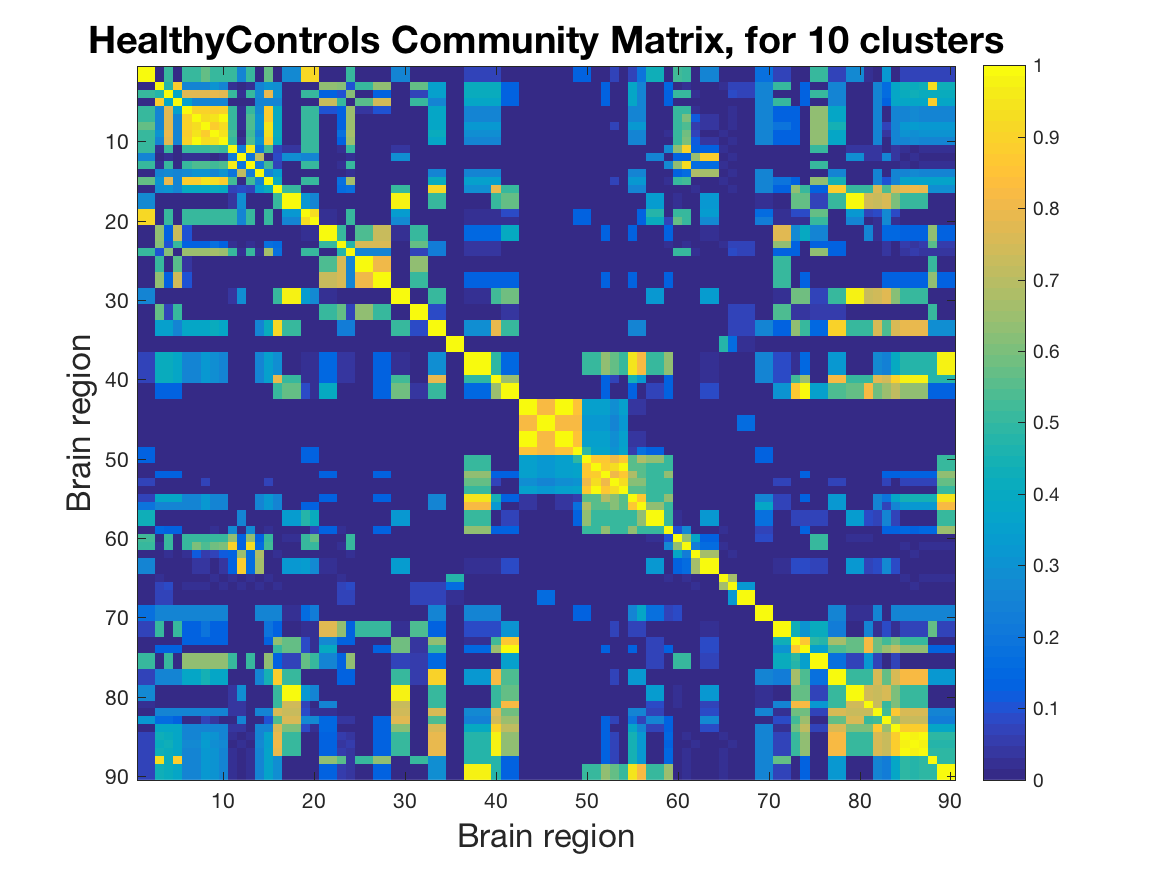
\includegraphics[width=\textwidth]{HealthyControls10.png}
		\caption{Healthy controls community matrix for 10 clusters}
		\label{fig:CM10healthy}
	\end{subfigure}
	\begin{subfigure}[b]{.49\textwidth}
		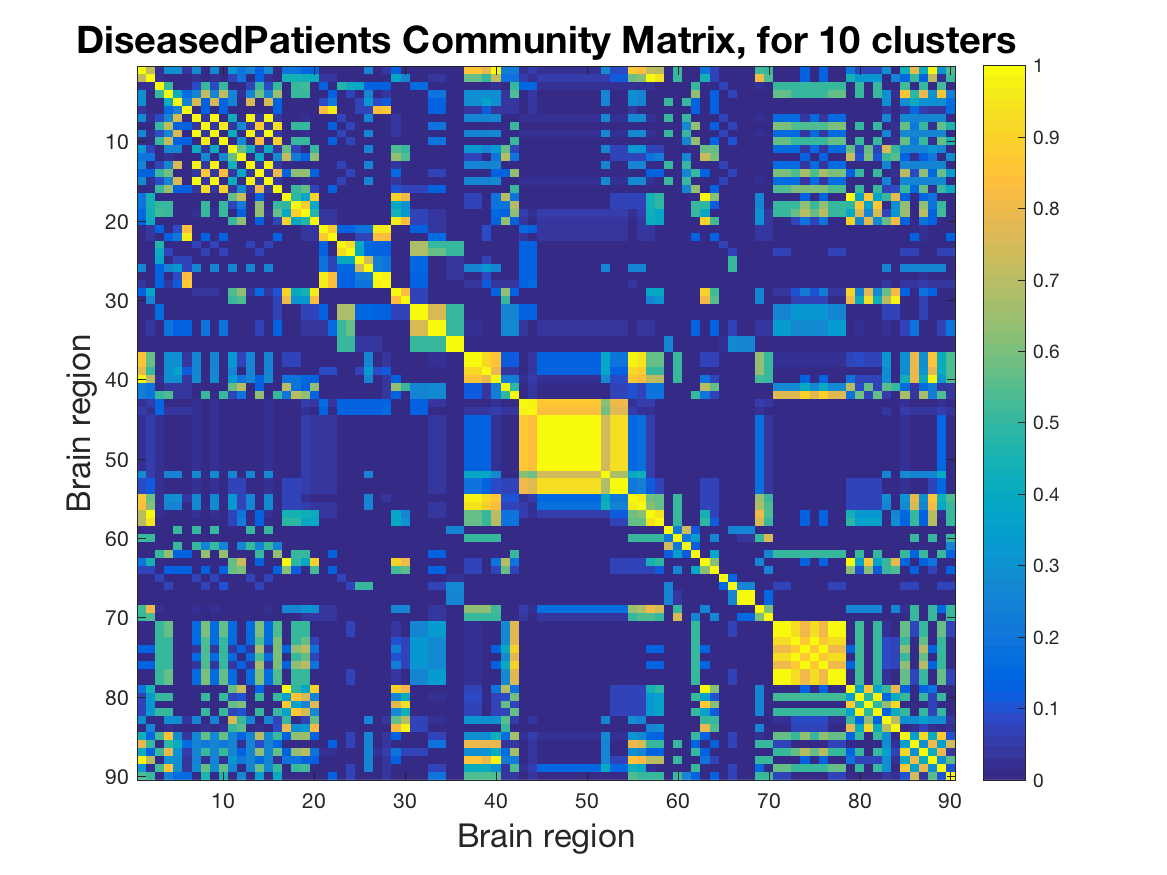
\includegraphics[width=\textwidth]{DiseasedPatients10.png}
		\caption{Diseased patients community matrix for 10 clusters}
		\label{fig:CM10diseased}
	\end{subfigure}
	\caption{Community matrices for 10 clusters}
	\label{fig:CM10}
\end{figure}

The `Difference Community Matrix' is the combined difference of the healthy controls and diseased patients. A yellow, or high value, indicates a strong connectivity in healthy controls, a blue, or low value, indicates a strong connectivity in diseased patients, and a green, or zero value, indicates there is equal connectivity between healthy and diseased patients. 

The difference matrix in Figure \ref{fig:CM10diff} illustrates that there is generally a stronger connectivity in healthy controls rather than in diseased patients.

\begin{figure}[h!] 
	\centering
	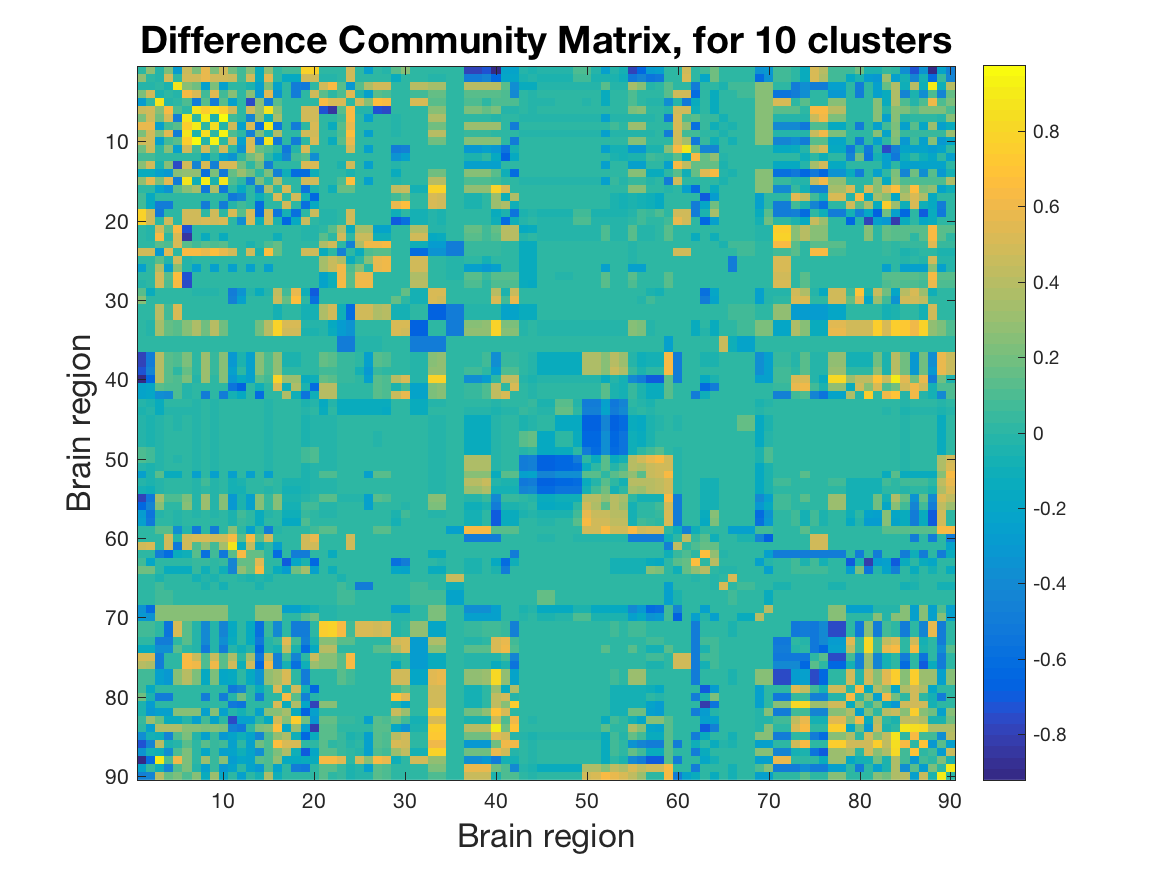
\includegraphics[width=\textwidth]{diffCommunityMatrix10.png}
	\caption{Difference community matrix for 10 clusters}
	\label{fig:CM10diff}
\end{figure}

\section{Results for 20 Clusters}
In this section we look at the same community matrices as described previously, but for a total of 20 clusters.

Looking at the healthy controls in Figure \ref{fig:CM20healthy} we can see strong connectivity consistently surrounding the diagonal. The diseased patients in Figure \ref{fig:CM20diseased} show similar results to before with the two same large blocks in the middle and bottom-right showing stronger connectivity across more brain regions. Interestingly, with 20 clusters less connectivity is shown in the far off diagonal brain regions in both Figures \ref{fig:CM20healthy} and \ref{fig:CM20diseased}.

\begin{figure}[h!] 
	\centering
	\begin{subfigure}[b]{.49\textwidth}
		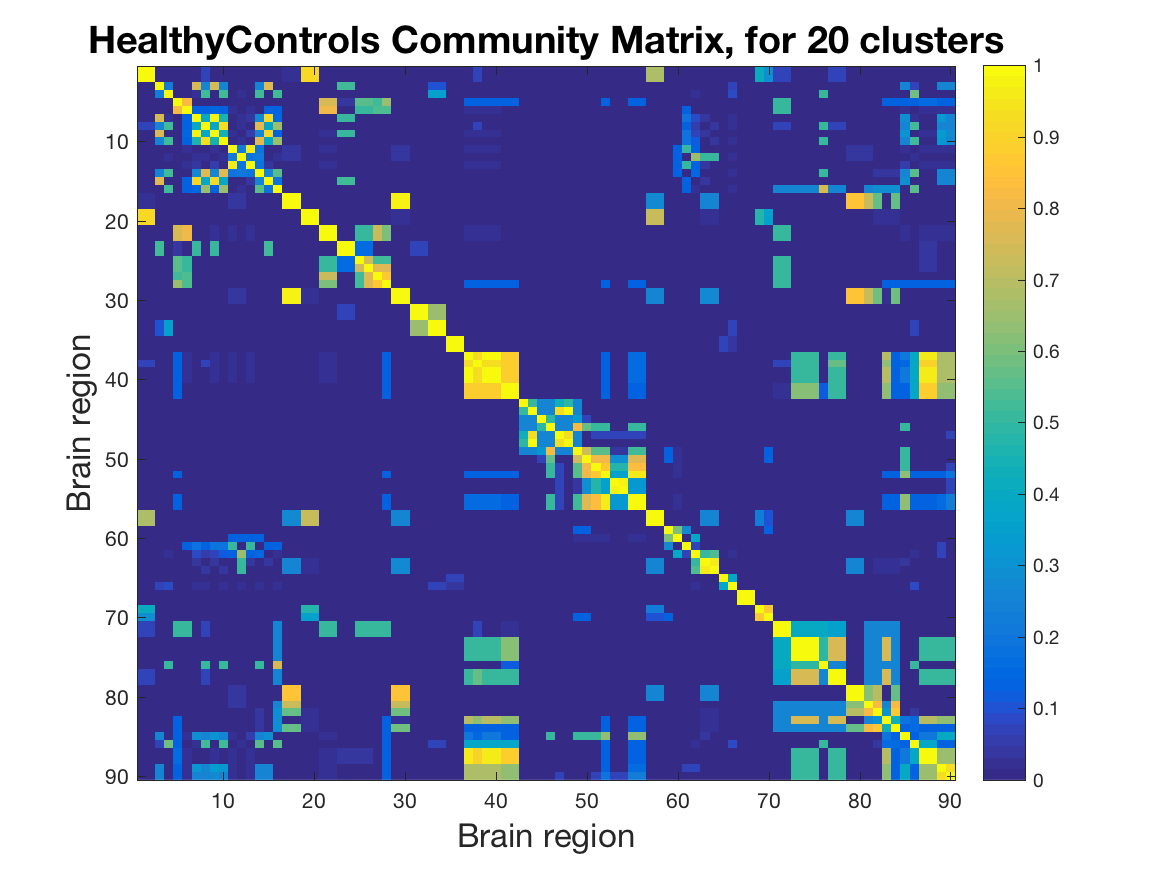
\includegraphics[width=\textwidth]{HealthyControls20.png}
		\caption{Healthy controls community matrix for 20 clusters}
		\label{fig:CM20healthy}
	\end{subfigure}
	\begin{subfigure}[b]{.49\textwidth}
		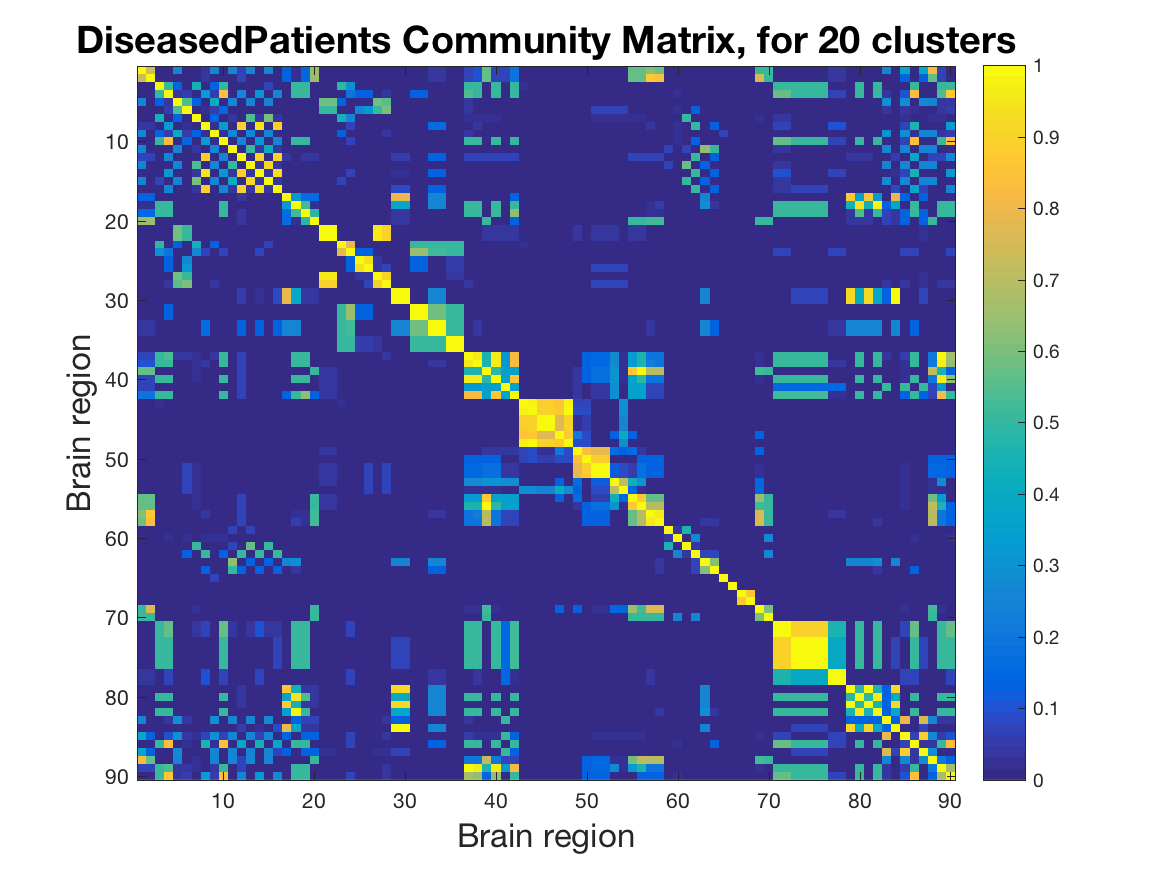
\includegraphics[width=\textwidth]{DiseasedPatients20.png}
		\caption{Diseased patients community matrix for 20 clusters}
		\label{fig:CM20diseased}
	\end{subfigure}
	\caption{Community matrices for 20 clusters}
	\label{fig:CM20}
\end{figure}

The difference matrix in Figure \ref{fig:CM20diff} illustrates that there is generally a stronger connectivity in healthy controls rather than in diseased patients but there are more strong connections for  less connectivity in far off diagonal brain regions. 

\begin{figure}[h!] 
	\centering
	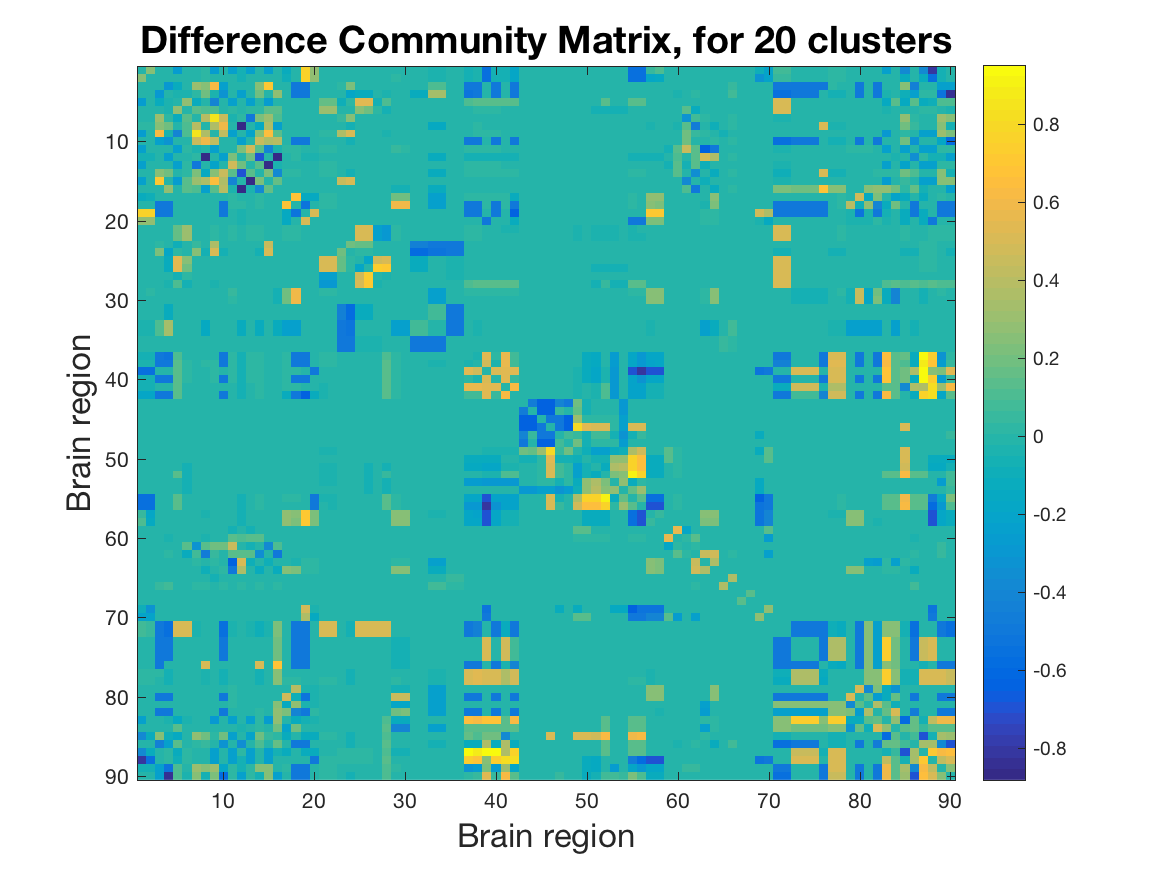
\includegraphics[width=\textwidth]{diffCommunityMatrix20.png}
	\caption{Difference community matrix for 20 clusters}
	\label{fig:CM20diff}
\end{figure}

\section{Results for 30 Clusters}
In this section we look at the same community matrices as described previously, but for a total of 30 clusters.

Performing k-means with 30 clusters yield similar results to 20 clusters, except possibly more refined. Looking at the healthy controls in Figure \ref{fig:CM30healthy} we can see vibrant yellows surround the diagonal as highlighted by the red boxes. The diseased patients in Figure \ref{fig:CM30diseased} show less strong connectivity occurring near the as shown by the middle two red boxes. The outer two boxes show that there is a decrease in the strength of connectivity but more connections with surrounding regions are made. As for 20 clusters, 30 clusters shows even less connectivity is shown in the far off diagonal brain regions as illustrated in both Figures \ref{fig:CM30healthy} and \ref{fig:CM30diseased}.

\begin{figure}[h!] 
	\centering
	\begin{subfigure}[b]{.49\textwidth}
		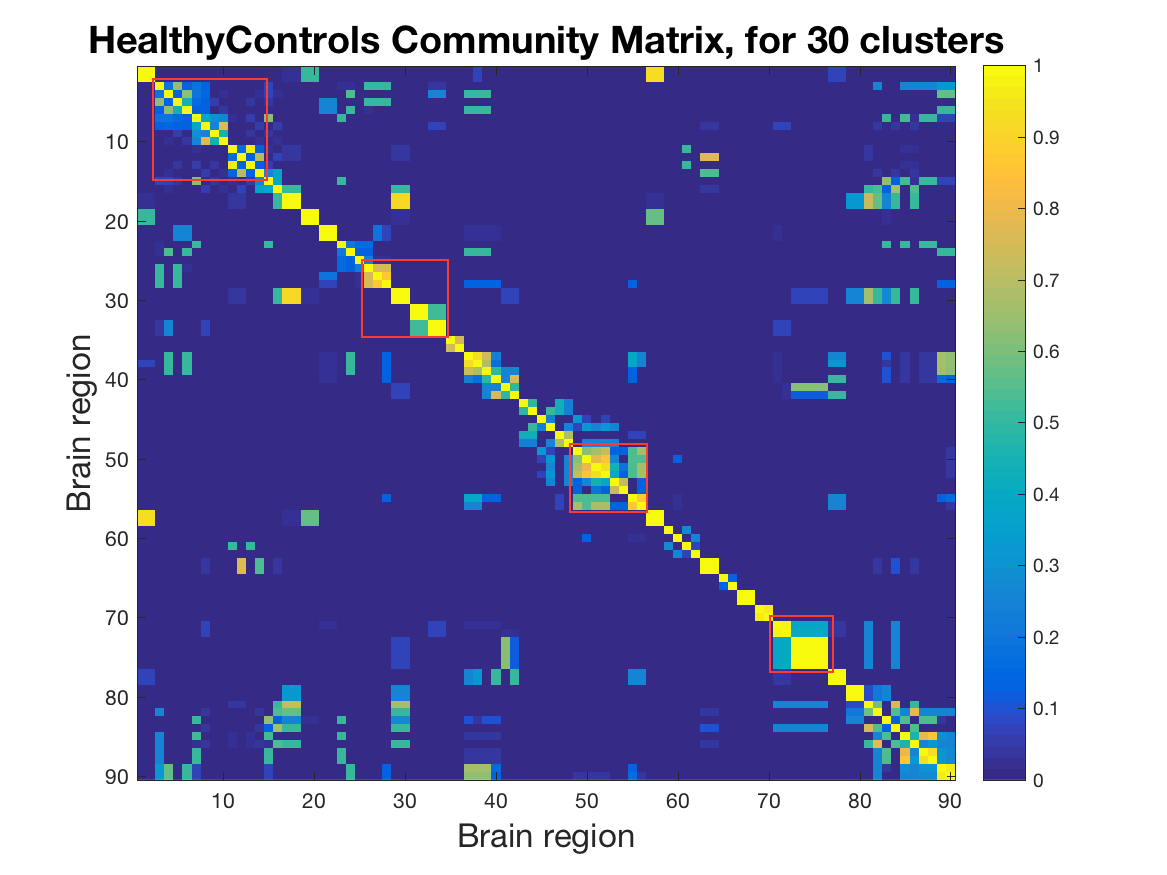
\includegraphics[width=\textwidth]{HealthyControls30.png}
		\caption{Healthy controls community matrix for 30 clusters}
		\label{fig:CM30healthy}
	\end{subfigure}
	\begin{subfigure}[b]{.49\textwidth}
		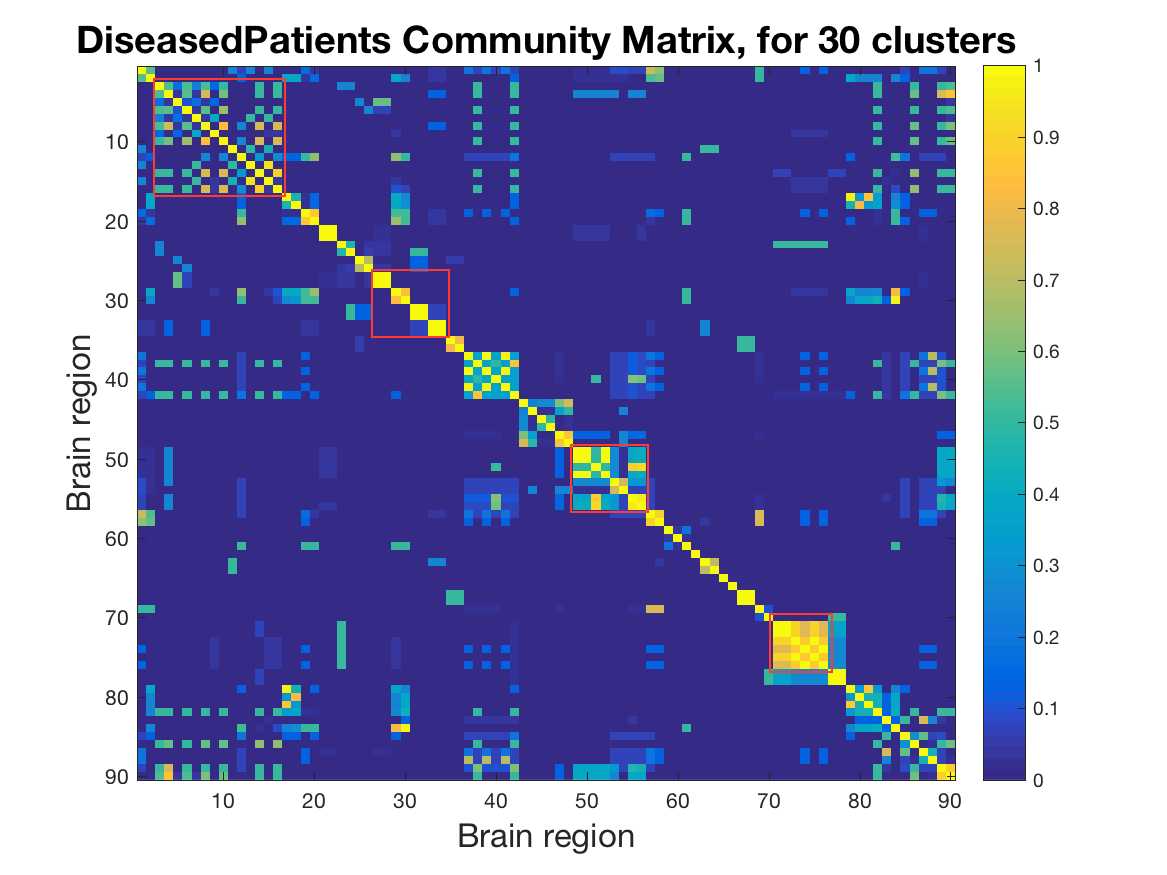
\includegraphics[width=\textwidth]{DiseasedPatients30.png}
		\caption{Diseased patients community matrix for 30 clusters}
		\label{fig:CM30diseased}
	\end{subfigure}
	\caption{Community matrices for 30 clusters}
	\label{fig:CM30}
\end{figure}

The difference matrix in Figure \ref{fig:CM30diff} shows that there is still stronger connectivity in the healthy controls, however, there are occurrences of distinct, strong, connections in diseased patients as highlighted by the red boxes.

\begin{figure}[h!] 
	\centering
	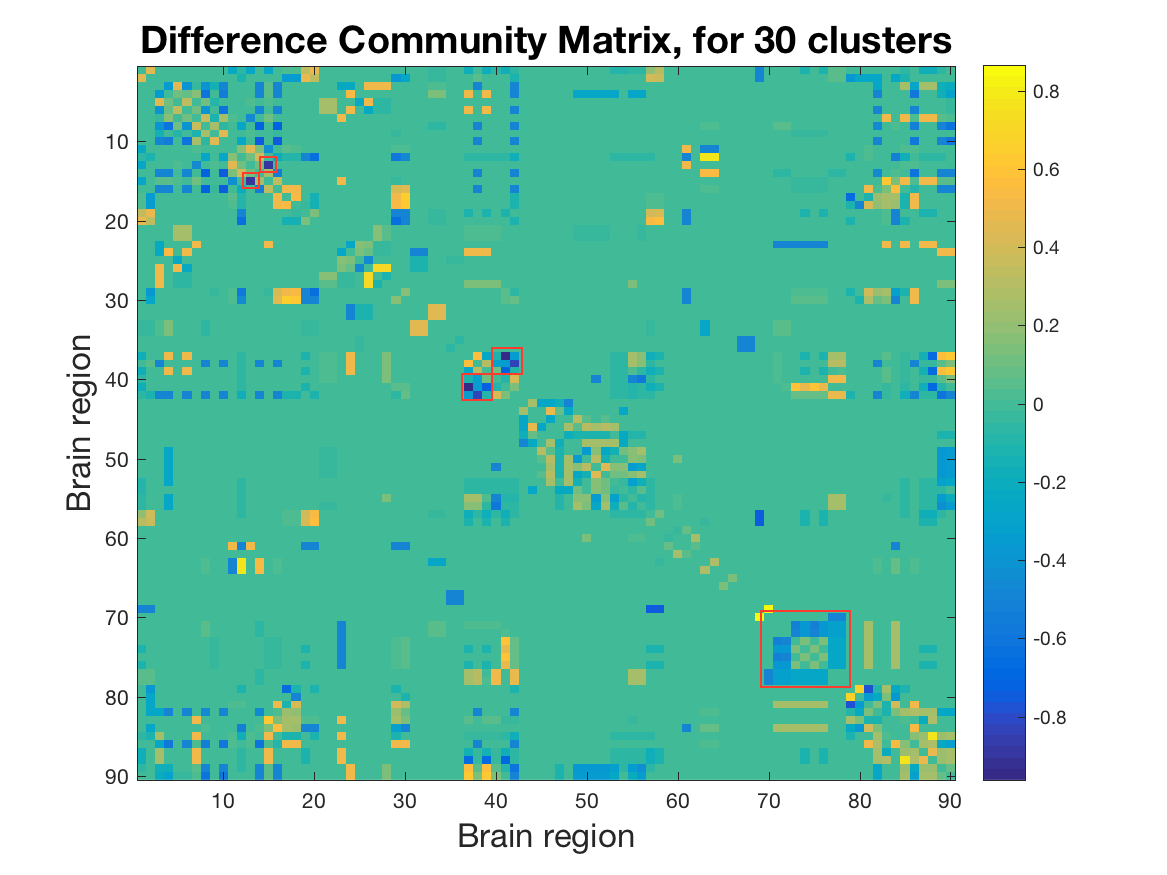
\includegraphics[width=\textwidth]{diffCommunityMatrix30.png}
	\caption{Difference community matrix for 30 clusters}
	\label{fig:CM30diff}
\end{figure}

\section{Comparison of number of clusters}
When comparing the results for the varying number of clusters we see a trend that there is less connectivity among the brain regions. This is evidenced by looking at the increase of 'blue' when looking at Figure \ref{fig:CM10} to \ref{fig:CM30}. In turn, this means only the brain regions with strong connectivity are highlighted. 

This occurrence can be explained by the number of clusters. With a lower number of clusters, there is more chance one brain region is in the same cluster as another. Conversely, there is a smaller chance of brain regions belonging to the same cluster with higher K. To explain further, if we assigned K to the number of brain regions, every region would belong to its own cluster and we would only see a yellow diagonal and blue off diagonal elements. On the other hand, if we assigned K to 1, every region would belong to the same cluster. Therefore, we can imagine there is an ideal balance for the value of K which highlights only the most similar (connected) brain regions. So, as we increase from 10 to 30 clusters, we filter out regions with weak connections and only the strong ones remain. This is useful for determining a pattern across the healthy and diseased patients as there is more distinction between the two classes.

Additionally, we can see a common pattern of connected brain regions as the number of clusters increase, albeit, it becomes more defined when K is 30.

\section{Comparison of community matrices}
This section is a comparison the community matrices for the healthy controls and the diseased patients, namely, the ones shown in \ref{fig:CM30}.

When looking at Figure \ref{fig:CM30healthy}, the healthy controls show a stronger coherence in neuro-activities across the two hemispheres surrounding the diagonal as depicted by the bright yellow squares. Interestingly in Figure \ref{fig:CM30diseased}, whilst the coherence is weaker, there are more connections in total as shown by the darker yellows highlighted in the red boxes. These could indicate that the disease weakens the connections between brain regions but allows more regions to connect. This may explain the adverse effects of the disease, as regions are functioning together when they never were originally.

\section{Further Comments}

In this section we look at finding the optimum number of clusters for identifying strong connectivity between brain regions.

\begin{figure}[h!] 
	\centering
	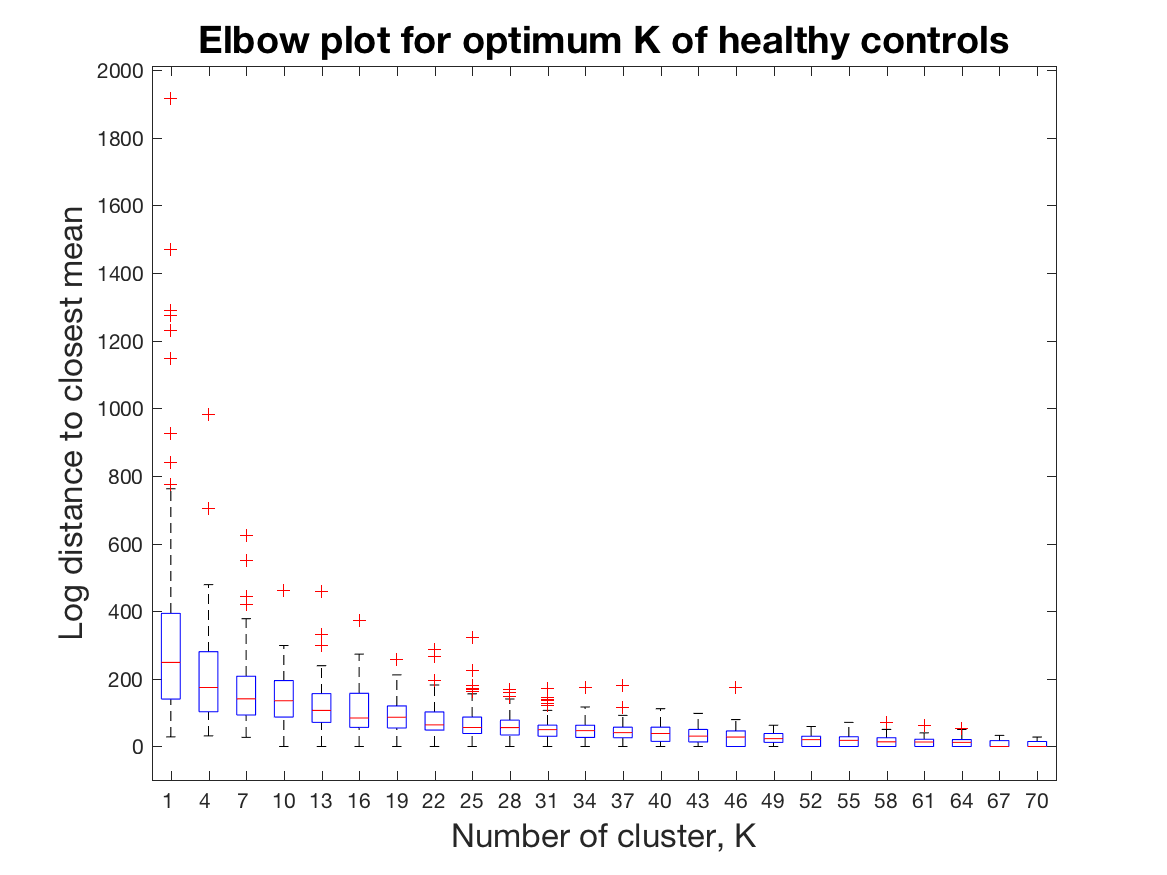
\includegraphics[width=\textwidth]{elbowHealthy.png}
	\caption{Elbow plot for healthy controls}
	\label{fig:ElbowHealthy}
\end{figure}

\begin{figure}[h!] 
	\centering
	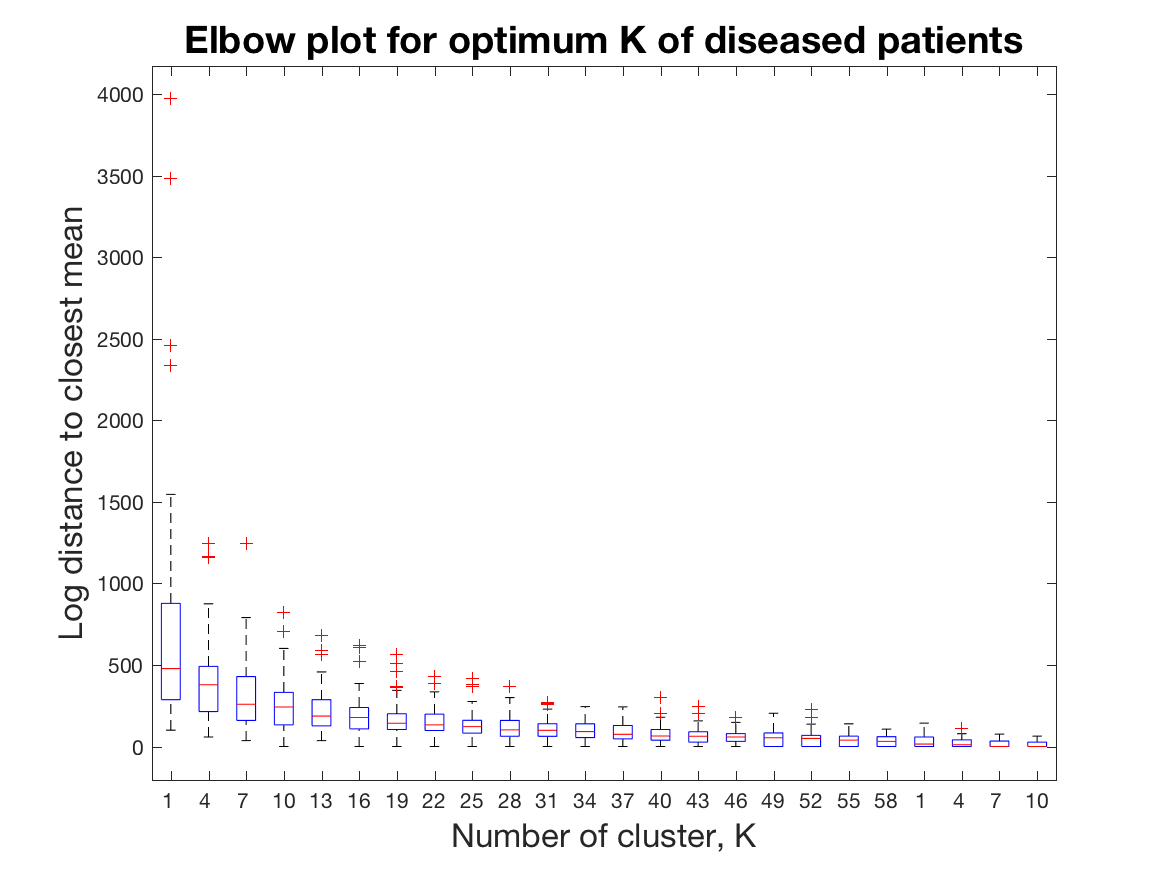
\includegraphics[width=\textwidth]{elbowDiseased.png}
	\caption{Elbow plot for diseased controls}
	\label{fig:ElbowDiseased}
\end{figure}










